% Ejemplo 1 de las diapositivas: BPA1 = 40; reinversión de 20 en t=2 (flujo 5 desde t=3) y de 27 en t=5 (flujo 5,40 desde t=6).
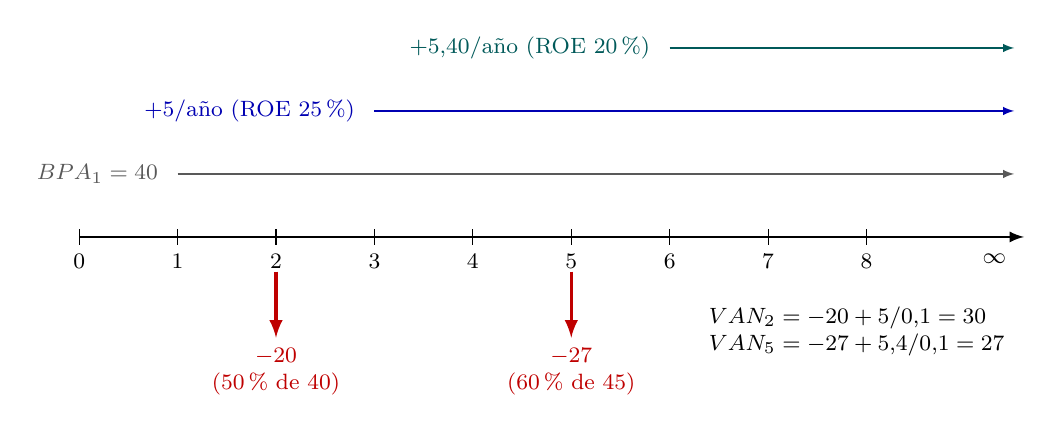
\begin{tikzpicture}[x=1.25cm, y=0.8cm, >=latex, font=\footnotesize]
  \draw[->, thick] (0,0) -- (9.6,0);
  \foreach \t in {0,...,8} { \draw (\t,0.12) -- (\t,-0.12) node[below] {$\t$}; }
  \node[below] at (9.3,-0.12) {$\infty$};
  % Beneficio de los activos actuales
  \draw[thick, gray!70!black] (1,1) -- (9.2,1); \node[anchor=east, gray!70!black] at (0.9,1) {$BPA_1 = 40$};
  \draw[->, gray!70!black] (9.2,1) -- (9.5,1);
  % Reinversión 1
  \draw[->, very thick, red!75!black] (2,-0.55) -- (2,-1.6) node[below, align=center] {$-20$\\(50\,\% de 40)};
  \draw[thick, blue!70!black] (3,2) -- (9.2,2); \draw[->, blue!70!black] (9.2,2) -- (9.5,2);
  \node[anchor=east, blue!70!black] at (2.9,2) {$+5$/año (ROE 25\,\%)};
  % Reinversión 2
  \draw[->, very thick, red!75!black] (5,-0.55) -- (5,-1.6) node[below, align=center] {$-27$\\(60\,\% de 45)};
  \draw[thick, teal!70!black] (6,3) -- (9.2,3); \draw[->, teal!70!black] (9.2,3) -- (9.5,3);
  \node[anchor=east, teal!70!black] at (5.9,3) {$+5{,}40$/año (ROE 20\,\%)};
  \node[anchor=west, font=\footnotesize, align=left] at (6.3,-1.5) {$VAN_2 = -20 + 5/0{,}1 = 30$\\$VAN_5 = -27 + 5{,}4/0{,}1 = 27$};
\end{tikzpicture}
